\documentclass[14pt]{book}
\usepackage[p,osf]{scholax}
\usepackage{amsfonts,amstext,amsbsy,amsopn,amsmath,eucal,bm,mathrsfs}
\usepackage[T1]{fontenc}
\usepackage{tgbonum}
\usepackage[scaled=1.075,ncf,vvarbb]{newtxmath}% need to scale up math package 
\normalfont
\usepackage[parfill]{parskip}% Begin paragraphs with an empty line rather than an indent

\usepackage{setspace,lineno,enumitem,fancyhdr,marginnote,hyperref}
\usepackage[capitalise]{cleveref}
\usepackage{pstool,pgfplots}
\usepackage[centering,text={18cm,22cm},showframe=false]{geometry}
\pagestyle{fancy}

\usepackage{wrapfig,graphicx,color,xcolor}
\usepackage[labelformat=empty]{caption}
\usepackage{multicol}
\usepackage{multirow}
\usepackage{booktabs}
\definecolor{light-gray}{gray}{0.96}
\definecolor{light-red}{rgb}{0.82, 0.1, 0.26}
\definecolor{light-smoke}{rgb}{0.96,0.96,0.93} 
\definecolor{light-olive}{rgb}{0.63,0.57,0.33} 
\definecolor{light-azul}{rgb}{0.25, 0.41, 0.88}
\definecolor{light-red}{rgb}{0.82, 0.1, 0.26}
\newcommand{\gc}[1]{\textcolor{light-azul}{#1}}
\newcommand{\rojo}[1]{\textcolor{light-red}{#1}}
\newcommand{\cita}[1]{\textcolor{light-azul}{\boxed{{\Large #1}}}}
\newcommand{\alp}[1]{\textcolor{light-azul}{\texttt{\quad#1}}}
\usepackage[pagecolor=light-gray]{pagecolor}

\usepackage{pythonhighlight}
\lstdefinelanguage{turtle}
{
    columns=fullflexible,
    keywordstyle=\color{light-red},
    morekeywords={@prefix,@base,@forSome,@forAll,@keywords},
    morecomment=[l]{\#},
    tabsize=4, 
    alsoletter={-?}, % allowed in names
    morecomment=[s][light-azul]{<}{>},
    basicstyle=\ttfamily\color{black}, 
    %numberstyle=\color{black},
    morestring=[b][\color{black}]\",    
    background=\color{light-gray},
 }
 
\usepackage{tikz}
\usetikzlibrary{matrix,chains,positioning,decorations.pathreplacing,arrows}
\usetikzlibrary{intersections,fit,arrows.meta,shapes.geometric}
\usetikzlibrary{calc}  
\tikzstyle{box} = [rectangle, minimum width=1.2cm, minimum height=1cm,text centered, draw=black, fill=white!30]
\tikzstyle{arrow} = [thick,->,>=stealth, blue!40]
\tikzstyle{circlex} = [circle, draw, thick, minimum size=1.2cm, inner sep=0, node distance=1cm, fill=white, path picture={\draw (path picture bounding box.south west) -- (path picture bounding box.north east) (path picture bounding box.south east) -- (path picture bounding box.north west);}]
\tikzstyle{circles} = [circle, draw, thick, minimum size=1.2cm, inner sep=0, node distance=1cm, fill=white]
\tikzstyle{triangled} = [regular polygon, regular polygon sides=3, draw, minimum size=1cm, node distance=1cm, fill=white, rotate=180, blue!40]
\tikzstyle{triangler} = [regular polygon, regular polygon sides=3, draw, minimum size=2em, node distance=1cm, fill=white, rotate=-90]
\tikzstyle{poligon} = [regular polygon, regular polygon sides=5, draw, minimum size=0.8cm, node distance=1cm, fill=blue!20]
\tikzstyle{textbox} = [rectangle, text width=6cm, text centered, draw=none]
\tikzstyle{hexagon} = [regular polygon, regular polygon sides=6, minimum size=3.5cm, text centered, draw=black, fill=blue!30]
\tikzstyle{block} = [rectangle, minimum width=3cm, minimum height=1cm, text centered, draw=black, fill=green!30]
\tikzstyle{mydiamond} = [draw, thick, shape=diamond, aspect=2, minimum width=3cm, minimum height=1.5cm, text centered, fill=yellow!30]
\tikzstyle{parallelogram} = [draw, thick, shape=trapezium, trapezium angle=75, minimum width=2.5cm, minimum height=1cm, text centered, fill=gray!30]
\tikzstyle{dashed_arrow} = [thick,dashed,->,>=stealth]

\usepackage{varwidth}
\usepackage{gnuplottex}
\usepackage[most]{tcolorbox}
\tcbset{colback=light-smoke, colframe=light-azul, 
	highlight math style= {enhanced, %<-- needed for the ’remember’ options
		colframe=light-olive,colback=light-smoke,boxsep=0pt}}


\providecommand{\promed}[1]{{\mathbb{E}}\left\lbrace #1\right\rbrace} 
\providecommand{\var}[1]{{\ensuremath{var}}\{#1\}}
\providecommand{\ve}[1]{{\boldsymbol {#1}}} %
\providecommand{\mat}[1]{{\pmb {#1}}} %
\providecommand{\est}[1]{{\widetilde {#1}}}
\newcommand{\Real}{\mathbb{R}}\newcommand{\N}{\mathbb{N}}
\providecommand{\s}[1]{\negthickspace#1\negthickspace}%
\def\checkmark{{\tikz\fill[scale=0.42](0,.36) -- (.24,0) -- (1,.72) -- (.24,.15) -- cycle;}\;}

\newcommand{\Cross}{$\mathbin{\tikz [x=1.4ex,y=1.4ex,line width=.2ex,  {light-red}] \draw (0,0) -- (1,1) (0,1) -- (1,0);}\;$}%
\def\halfcheckmark{\tikz\draw[scale=0.4,fill=orange](0,.35) -- (.25,0) -- (1,.7) -- (.25,.15) -- cycle (0.75,0.2) -- (0.77,0.2)  -- (0.6,0.7) -- cycle;\;\;}
\usepackage{titlesec}
\titleformat{\section}[block]{\color{light-azul}\Large\bfseries\filcenter}{}{1em}{}
\titleformat{\subsection}[hang]{\bfseries}{}{1em}{}
\titleformat{\subsubsection}[hang]{\scshape\filcenter}{}{1em}{}

\setlength{\fboxrule}{1.2pt}

\newenvironment{DefQuot}[2]{%
	\upshape\begin{spacing}{#1}
		\centering
		\fcolorbox{light-azul}{light-smoke}{
			\parbox{.75\textwidth}{ 
				{
					{#2}
		}}}
	}{%
	\end{spacing}
}

\newenvironment{Example}[3]{%
	\upshape\begin{spacing}{#1}
		\fcolorbox{light-olive}{light-smoke}{
			\parbox{.48\textwidth}{ 
				{
					{ #2}
		}}}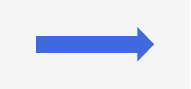
\begin{tikzpicture}
	\color{light-azul}
	\draw[-{Triangle[width=12pt,length=6pt]}, line width=6pt](0,0) -- (1.5, 0);
\end{tikzpicture}{\color{light-azul}{\Large #3}}
	}{%
	\end{spacing}
}

\newenvironment{Tasks}[1]{%
	\upshape\begin{spacing}{1.5}
				\centering
		\fcolorbox{black}{white}{
			\parbox{.96\textwidth}{ 
				{
					{\fontfamily{lmr}\selectfont #1}
		}}}
	}{%
	\end{spacing}
}
\usepackage{enumitem}
\usepackage{multirow}
\usepackage{booktabs}
 
%%%%%%%%%%%%%%%%%%%%%%%%%%%%%%%%%%%%%%%%%%%%%%%%%%%%%%%%%%%%
\newcommand{\courseName}{\emph{Spectrum~Sensing~System
}} 
% Insert course name here
\title{\courseName}

% Headers and footers. See documentation for 'fancyhdr' package for more information.
\lhead{\scriptsize\fontfamily{lmr}\courseName} % Left header
% Center header
\rhead{\thepage} % Right header
\lfoot{} % Left footer
\cfoot{\scriptsize\fontfamily{lmr} Electronics and Computing, UNAL, Manizales} % Center footer
\rfoot{} % Right footer
%%%%%%%%%%%%%%%%%%%%%%%%%%%%%%%%%%%%%%%%%%%%%%%%%%%%%%%%%%%%
\providecommand{\H}{\texttt{HackRF~One}}
 
\usepackage{svg} 
\begin{document}
\maketitle
\thispagestyle{fancy}

\section{High-Level Tasks in Cognitive Radio and Spectrum Sensing}

\subsection{Power Spectral Density (PSD) Estimation}
This task involves estimating the distribution of power across different frequency components of a signal. It is fundamental to understanding the spectral characteristics of the observed environment.

\begin{enumerate}
	\item \textbf{Spectral Parameter Estimation.} Key features derived from the PSD include:
	\begin{itemize}
		\item Peak frequencies (locations of maximum power),
		\item Bandwidth (range of occupied frequencies),
		\item Power levels at specific frequencies,
		\item Center frequency (mean spectral centroid).
	\end{itemize}
	
	\item \textbf{Quantitative Reconstruction of PSD.} This involves reconstructing the original PSD from noisy or undersampled data using techniques such as interpolation, smoothing, or model-based estimation.
	
	\item \textbf{Demodulation Support.} PSD estimation assists in identifying carrier frequencies and modulation schemes, facilitating demodulation of the received signals.
\end{enumerate}

\subsection{Signal Detection}
This task focuses on determining the presence of informative content within the received signal.

\begin{enumerate}
	\item \textbf{Detection of Signal Presence (Thresholding).} A threshold is applied to a test statistic (e.g., energy) to decide whether a signal is present.
	
	\item \textbf{Symbol Detection.} Once signal presence is confirmed, the next step is identifying the transmitted symbols, such as bits in digital communication systems.
\end{enumerate}

\subsection{Identification and Classification of Signals}
This task involves characterizing signals based on observed features.

\begin{enumerate}
	\item \textbf{Modulation Classification.} Determining the modulation format (e.g., AM, FM, QAM, PSK) is critical for enabling correct demodulation and decoding.
	
	\item \textbf{Spatio-Temporal Identification of Spurious Signals.} This involves localizing and characterizing unwanted signals across both spatial and temporal domains.
	
	\item \textbf{Spatio-Temporal Identification of Interference.} Identifying and profiling interference sources that affect the desired signal, considering their spatio-temporal evolution.
\end{enumerate}

\subsection{Channel State Estimation}
Characterizing the wireless channel is essential for compensating for impairments such as fading or noise.

\begin{enumerate}
	\item \textbf{Channel Impulse Response (CIR).} Estimation of how the channel distorts the temporal profile of the signal.
	
	\item \textbf{Channel Frequency Response (CFR).} Estimation of the channel's effect on signal amplitude and phase across frequency.
\end{enumerate}

\subsection{Decision-Making}
Based on the outcomes of the previous steps, appropriate decisions are made to complete the communication or control loop.

\begin{enumerate}
	\item Decoding of the received data.
	\item Choosing an optimal action in adaptive or control-oriented systems.
	\item Interference identification and mitigation strategies.
\end{enumerate}

\section{Recent Civilian-Focused RF Spectrum Sensing Systems}

\begin{table}[h]
	\centering
	\begin{tabular}{@{}lll@{}}
		\toprule
		\textbf{System} & \textbf{Year} & \textbf{Application Focus} \\
		\midrule
		GBSense & 2024 & \begin{tabular}[c]{@{}l@{}}Wideband RF spectrum monitoring with low-cost\\setup. Utilizes sub-Nyquist sampling for real-\\time analysis.\end{tabular} \\
		\addlinespace
		Compressed-Sensing & 2024 & \begin{tabular}[c]{@{}l@{}}Real-time RF emitter detection and localization\\for non-cooperative civilian radio monitoring\\using compressed sensing.\end{tabular} \\
		Localization System & & \\
		\bottomrule
	\end{tabular}
	\caption{Recent civilian-focused RF spectrum sensing systems developed since 2024.}
	\label{tab:recent_systems}
\end{table}

\section{Implementation Details of GBSense: A GHz-Bandwidth Compressed Spectrum Sensing System}

\subsection{Core Architecture and Sampling Strategy}

\begin{itemize}
	\item \textbf{Periodic Non-Uniform Sampling via Time-Interleaved ADC (TI-ADC):} Utilizes multiple ADC lanes operating in parallel, interleaved in time, to form structured non-uniform sampling patterns. Enables capture of up to 2 GHz of RF bandwidth with only 400 MHz average sampling rate.
	
	\item \textbf{Clock Distribution and Synchronization:} A dedicated subsystem ensures precise timing across ADC channels, mitigating jitter and preserving temporal alignment.
\end{itemize}

\subsection{Hardware Components}

\begin{itemize}
	\item \textbf{Power Splitter Subsystem:} Distributes incoming RF signals to multiple ADC lanes for parallel capture.
	
	\item \textbf{Time-Interleaved Sampling Subsystem:} Incorporates off-the-shelf ADC modules phased across time to support sub-Nyquist sampling.
	
	\item \textbf{Logic Device Subsystem:} FPGA or microcontroller-based logic handles sample alignment, decimation, buffering, and transmission to the host processor.
\end{itemize}

\subsection{Real-Time Software Integration}

\begin{itemize}
	\item \textbf{Low-Power Processor:} A Raspberry Pi processes ADC output for spectral reconstruction using compressed sensing algorithms.
	
	\item \textbf{Software Pipeline:}
	\begin{enumerate}
		\item Data decimation and formatting,
		\item Compressed sensing-based spectrum reconstruction,
		\item Spectral detection via thresholding.
	\end{enumerate}
	
	\item \textbf{Latency:} Real-time spectrum sensing achieved with $\sim$30 ms frame processing latency.
\end{itemize}

\subsection{Performance Metrics}

\begin{itemize}
	\item \textbf{Detection Accuracy:}
	\begin{itemize}
		\item 100\% accuracy for spectrum occupancy below 100 MHz,
		\item Over 80\% accuracy for 200 MHz occupancy levels.
	\end{itemize}
	
	\item \textbf{Throughput:} Frame-wise analysis completed in under 30 ms.
\end{itemize}

\subsection{System Design Innovations}

\begin{itemize}
	\item \textbf{Hardware-Friendly Design:} Avoids analog delay lines typical in multicoset architectures; instead, uses programmable digital timing via TI-ADC.
	
	\item \textbf{Adaptive Sampling Pattern Control:} Sampling patterns are programmable, allowing adaptation to varying spectral environments.
	
	\item \textbf{Modular and Cost-Efficient:} Constructed with commercially available components and low-cost processing, suitable for scalable and field-deployable applications.
\end{itemize}

\subsection{Summary of Key Specifications}

\begin{table}[h]
	\centering
	\begin{tabular}{@{}ll@{}}
		\toprule
		\textbf{Feature} & \textbf{Specification} \\
		\midrule
		RF Bandwidth & 2 GHz \\
		Average Sampling Rate & 400 MHz \\
		ADC Methodology & Time-Interleaved ADC (TI-ADC) \\
		Processor & Raspberry Pi \\
		Frame Processing Latency & $\sim$30 ms \\
		Detection Accuracy @ $<$100 MHz Occupancy & 100\% \\
		Detection Accuracy @ 200 MHz Occupancy & $>$80\% \\
		\bottomrule
	\end{tabular}
	\caption{Key technical characteristics of the GBSense system.}
	\label{tab:gbsense_specs}
\end{table}

\section{Implementation Details of the Compressed-Sensing Localization System}

\subsection{System Overview}
A prototype designed for real-time monitoring and localization of non-cooperative RF emitters, using compressed sensing combined with TDoA (Time Difference of Arrival) measurements.

\subsection{Hardware Architecture}

\begin{itemize}
	\item \textbf{Multiple Sensing Nodes:} Distributed SDR units capture wideband RF signals.
	
	\item \textbf{Compressed Sampling at Nodes:} Each node applies a measurement matrix (e.g., Gaussian) to compress incoming signals before transmission to a fusion center.
	
	\item \textbf{Fusion Node:} Collects compressed samples from nodes and performs joint reconstruction and localization.
\end{itemize}

\subsection{Signal Processing Pipeline}

\begin{enumerate}
	\item \textbf{Compressed Sensing Reconstruction:} Implements greedy algorithms (e.g., OMP) or convex recovery to reconstruct wideband signals from undersampled measurements.
	
	\item \textbf{TDoA Estimation:} Uses the reconstructed signals at multiple nodes to extract arrival-time differences for source localization.
	
	\item \textbf{Localization Algorithm:} Estimates emitter coordinates using TDoA multilateration based on reconstructed timing differences.
\end{enumerate}

\subsection{Software and Computational Aspects}

\begin{itemize}
	\item \textbf{Localization Logic:} Fusion center runs CS recovery and TDoA multilateration algorithms in real time.
	
	\item \textbf{Mapping Interface:} Localization results are displayed on a digital/interactive map, even in offline settings.
\end{itemize}

\subsection{Performance and Evaluation}

\begin{itemize}
	\item \textbf{Sample Compression Ratio:} Significant data reduction at nodes via CS before transmission.
	
	\item \textbf{Detection Performance:} ROC curves indicate that CS-enabled sensing achieves performance comparable to full-rate sampling even at moderate SNRs.
	
	\item \textbf{Localization Accuracy:} TDoA-based multilateration yields precise emitter positions; specific error metrics vary by node geometry and quality.
\end{itemize}

\subsection{Innovations and Advantages}

\begin{itemize}
	\item \textbf{Efficient Use of Bandwidth:} Combines sub-Nyquist sampling and compressed sensing to reduce node-to-fusion bandwidth.
	
	\item \textbf{Scalable Architecture:} Easily extensible by adding SDR nodes to improve localization precision.
	
	\item \textbf{Real-Time Mapping:} Integration with digital map interfaces enables near real-time emitter tracking.
\end{itemize}

\subsection{Key Specifications and Summary}

\begin{table}[h]
	\centering
	\begin{tabular}{@{}ll@{}}
		\toprule
		\textbf{Feature} & \textbf{Specification} \\
		\midrule
		Number of Nodes & Multiple SDR-based sensing units \\
		Sampling Technique & \begin{tabular}[c]{@{}l@{}}Compressed sensing (e.g., using random\\Gaussian projections)\end{tabular} \\
		Signal Recovery & Greedy (OMP) or convex CS algorithms \\
		Localization Method & TDoA multilateration on reconstructed signals \\
		Interface & Real-time display on digital/offline map \\
		Performance & \begin{tabular}[c]{@{}l@{}}ROC curves similar to full-rate systems\\at moderate SNR\end{tabular} \\
		\bottomrule
	\end{tabular}
	\caption{Technical summary of the compressed-sensing localization system.}
	\label{tab:cs_localization_specs}
\end{table}

\section{Similar Spectrum Sensing Systems from 2024}

\subsection{Commercial and Industrial Systems}

\subsubsection{Anritsu-DeepSig AI-Based RF Sensing Solution}
\textbf{Release:} Demonstrated at Mobile World Congress 2024

\textbf{System Overview:} Integration of Anritsu MS2090A Field Master Pro Spectrum Analyzer with DeepSig's AI-powered wireless signal detection and classification software. Employs deep learning, data-driven approach to rapidly incorporate new radio signal models using DeepSig's ML training tools.

\textbf{Key Features:}
\begin{itemize}
	\item \textbf{AI-Native Architecture:} Built on patented artificial intelligence deep learning algorithms
	\item \textbf{Rapid Signal Learning:} RF signals of interest from diverse new sources like drones and IoT devices can be learned quickly and accurately in days rather than months
	\item \textbf{Real-Time Adaptation:} Enables real-time adaptation to changing RF conditions
	\item \textbf{6G Readiness:} Forms foundation for AI-native RF sensing for 6G networks
\end{itemize}

\textbf{Applications:}
\begin{itemize}
	\item Spectrum awareness and optimization
	\item Network performance enhancement
	\item Dynamic spectrum sharing
	\item IoT and drone signal detection
\end{itemize}

\subsubsection{CRFS RFeye Node Plus Series}
\textbf{Release:} Enhanced models introduced throughout 2024

\textbf{System Overview:} Powerful, portable, and rugged RF sensors built for any environment that receive and record signals and geolocation of transmitters. Ultra-wide frequency, high-performance radio direction finding that synchronously uses TDoA and DF techniques.

\textbf{Key Features:}
\begin{itemize}
	\item \textbf{Multi-Technique Localization:} Combined Time Difference of Arrival (TDoA) and Direction Finding (DF)
	\item \textbf{Wide Frequency Coverage:} Ultra-wideband RF sensing capabilities
	\item \textbf{Environmental Ruggedness:} Designed for harsh operational environments
	\item \textbf{Real-Time Processing:} Allow users to see who is using the spectrum, where and when they are using it, and what they are using it for
\end{itemize}

\subsection{Academic and Research Systems}

\subsubsection{Deep Learning-Based Compressed Spectrum Sensing Systems}
\textbf{Publication:} Multiple IEEE papers published in 2024

\textbf{System Overview:} Compressive spectrum sensing (CSS) systems critical for efficient wideband spectrum sensing (WSS) using deep learning approaches. Wideband signal CS reconstruction algorithm by merging iterative shrinkage thresholding with deep learning.

\textbf{Key Features:}
\begin{itemize}
	\item \textbf{Sub-Nyquist Sampling:} Efficient wideband sensing with reduced sampling rates
	\item \textbf{Deep Learning Integration:} CNN and RNN-based signal reconstruction
	\item \textbf{Adaptive Sparsity:} Handles unknown and dynamically changing sparsity orders
	\item \textbf{Reduced Complexity:} Eliminates hand-crafted optimization parameters
\end{itemize}

\subsubsection{Multiband SDR-Based Spectrum Sensing Systems}
\textbf{Publication:} Enhanced implementations published in 2024

\textbf{System Overview:} Novel multiband spectrum sensing technique based on multiresolution analysis (wavelets), machine learning, and the Higuchi fractal dimension. Real-time implementation using affordable software-defined radios.

\textbf{Key Features:}
\begin{itemize}
	\item \textbf{Multiband Capability:} Simultaneous sensing across multiple frequency bands
	\item \textbf{Machine Learning Integration:} Wavelet-based feature extraction with ML classification
	\item \textbf{Cost-Effective:} Uses affordable SDR platforms
	\item \textbf{Modular Design:} Linkable SDR units for wide-band coverage
\end{itemize}

\subsection{Key Trends and Innovations in 2024}

\subsubsection{Common Characteristics}
\begin{enumerate}
	\item \textbf{AI/ML Integration:} Most systems incorporate deep learning or machine learning
	\item \textbf{Real-Time Processing:} Emphasis on low-latency, real-time operation
	\item \textbf{Compressed Sensing:} Widespread adoption of sub-Nyquist sampling techniques
	\item \textbf{Cooperative Networks:} Distributed sensing with centralized fusion
	\item \textbf{SDR-Based Platforms:} Cost-effective software-defined radio implementations
	\item \textbf{Multi-Band Capability:} Simultaneous sensing across multiple frequency bands
\end{enumerate}

\subsubsection{Technical Advances}
\begin{itemize}
	\item \textbf{Improved Reconstruction:} Deep learning-based signal reconstruction
	\item \textbf{Adaptive Algorithms:} Self-configuring parameters and sparsity handling
	\item \textbf{Enhanced Localization:} Combined TDoA/DF techniques for precise geolocation
	\item \textbf{Reduced Complexity:} Streamlined algorithms for real-time deployment
	\item \textbf{Better Accuracy:} Superior performance in challenging RF environments
\end{itemize}

\subsubsection{Application Focus}
\begin{itemize}
	\item Civilian spectrum monitoring and compliance
	\item IoT and drone signal detection
	\item 5G/6G network optimization
	\item Interference detection and mitigation
	\item Regulatory enforcement support
\end{itemize}

\section{Implementation}

\subsection{Power Spectral Density (PSD) Estimation}
This task involves estimating the distribution of power across different frequency components of a signal. It is fundamental to understanding the spectral characteristics of the observed environment.
	\begin{itemize}
		\item Peak frequencies (locations of maximum power),
		\item Bandwidth (range of occupied frequencies),
		\item Power levels at specific frequencies,
		\item Center frequency (mean spectral centroid).
	\end{itemize}
	
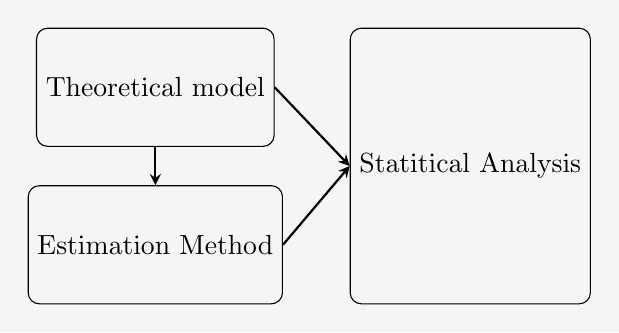
\begin{tikzpicture}
	% Define box styles
	\tikzstyle{box} = [draw, rectangle, rounded corners, minimum width=3cm, minimum height=1.5cm]
	\tikzstyle{arrow} = [->, >=stealth, thick]
	
	% Define box positions
	\node (box1) at (0,2) [box] {Theoretical model};
	\node (box2) at (0,0) [box] {Estimation Method};
	\node (box34) at (4,1) [box, minimum height=3.5cm] {Statitical Analysis}; % Merged box, centered vertically
	
	% Connect boxes with arrows horizontally
	\draw [arrow] (box1.east) -- (box34.west);
	\draw [arrow] (box2.east) -- (box34.west);
	
	% Add arrow from top right to bottom right of box34
	\draw [arrow] (box1.south) -- (box2.north);
\end{tikzpicture}
 
	
	
\end{document}

